%======================================================================
\chapter[Mechanical Drawings]{Mechanical CAD Drawings}
%======================================================================
\label{app:drawings}

The following drawings detail the complete mechanical design of a 14 DOF bipedal robot and supporting frame developed for experimental validation.  

\section{Bipedal Robot}
\label{app:bipedcad}
The 14 DOF bipedal robot was designed with DC motors from Micromo\footnote{http://www.micromo.com} and drivetrain components from Misumi USA\footnote{http://www.misumiusa.com}. 

% \begin{figure}[!h]
% 	\begin{center}
%     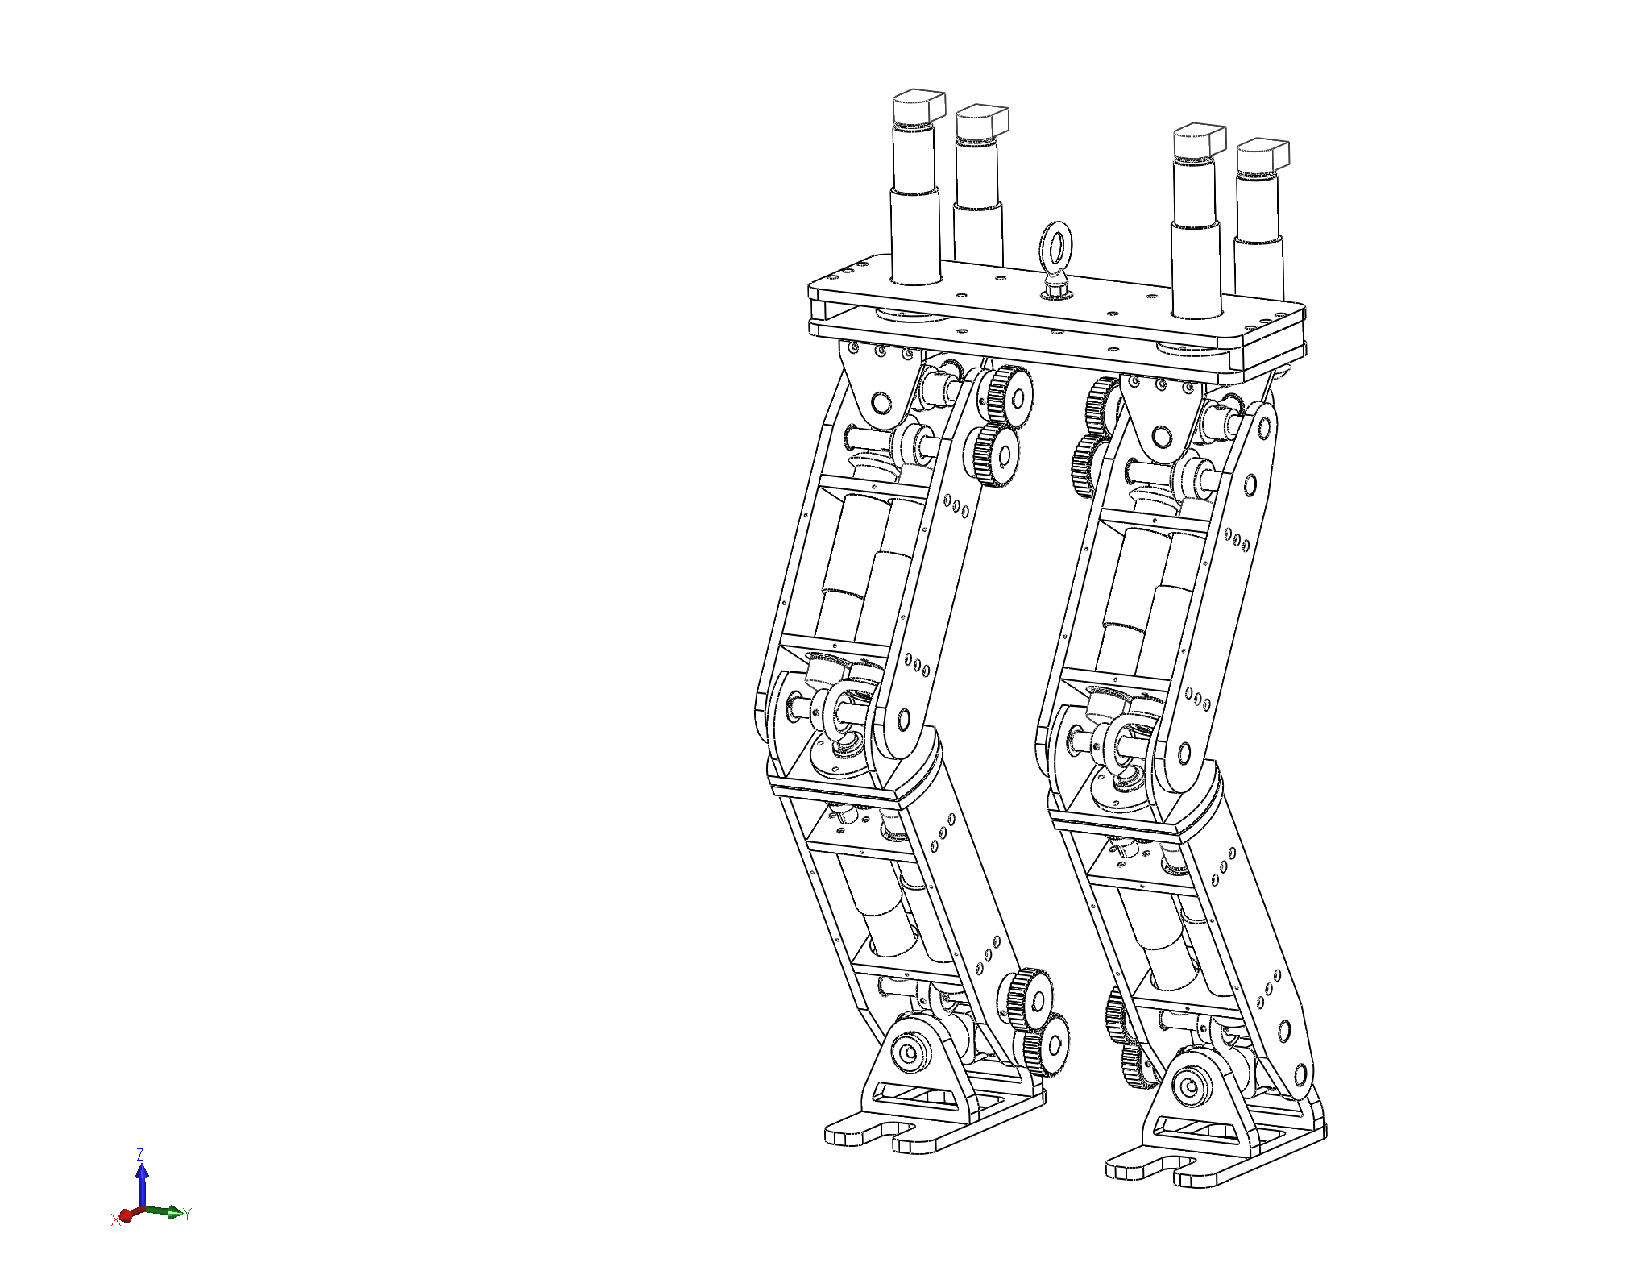
\includegraphics[trim = 5mm 20mm 5mm 5mm,clip,width=5cm]{fig/drawings/aslhp-biped.pdf}
% 	\end{center}
% \end{figure}

\begin{figure}[!h]
	\begin{center}
    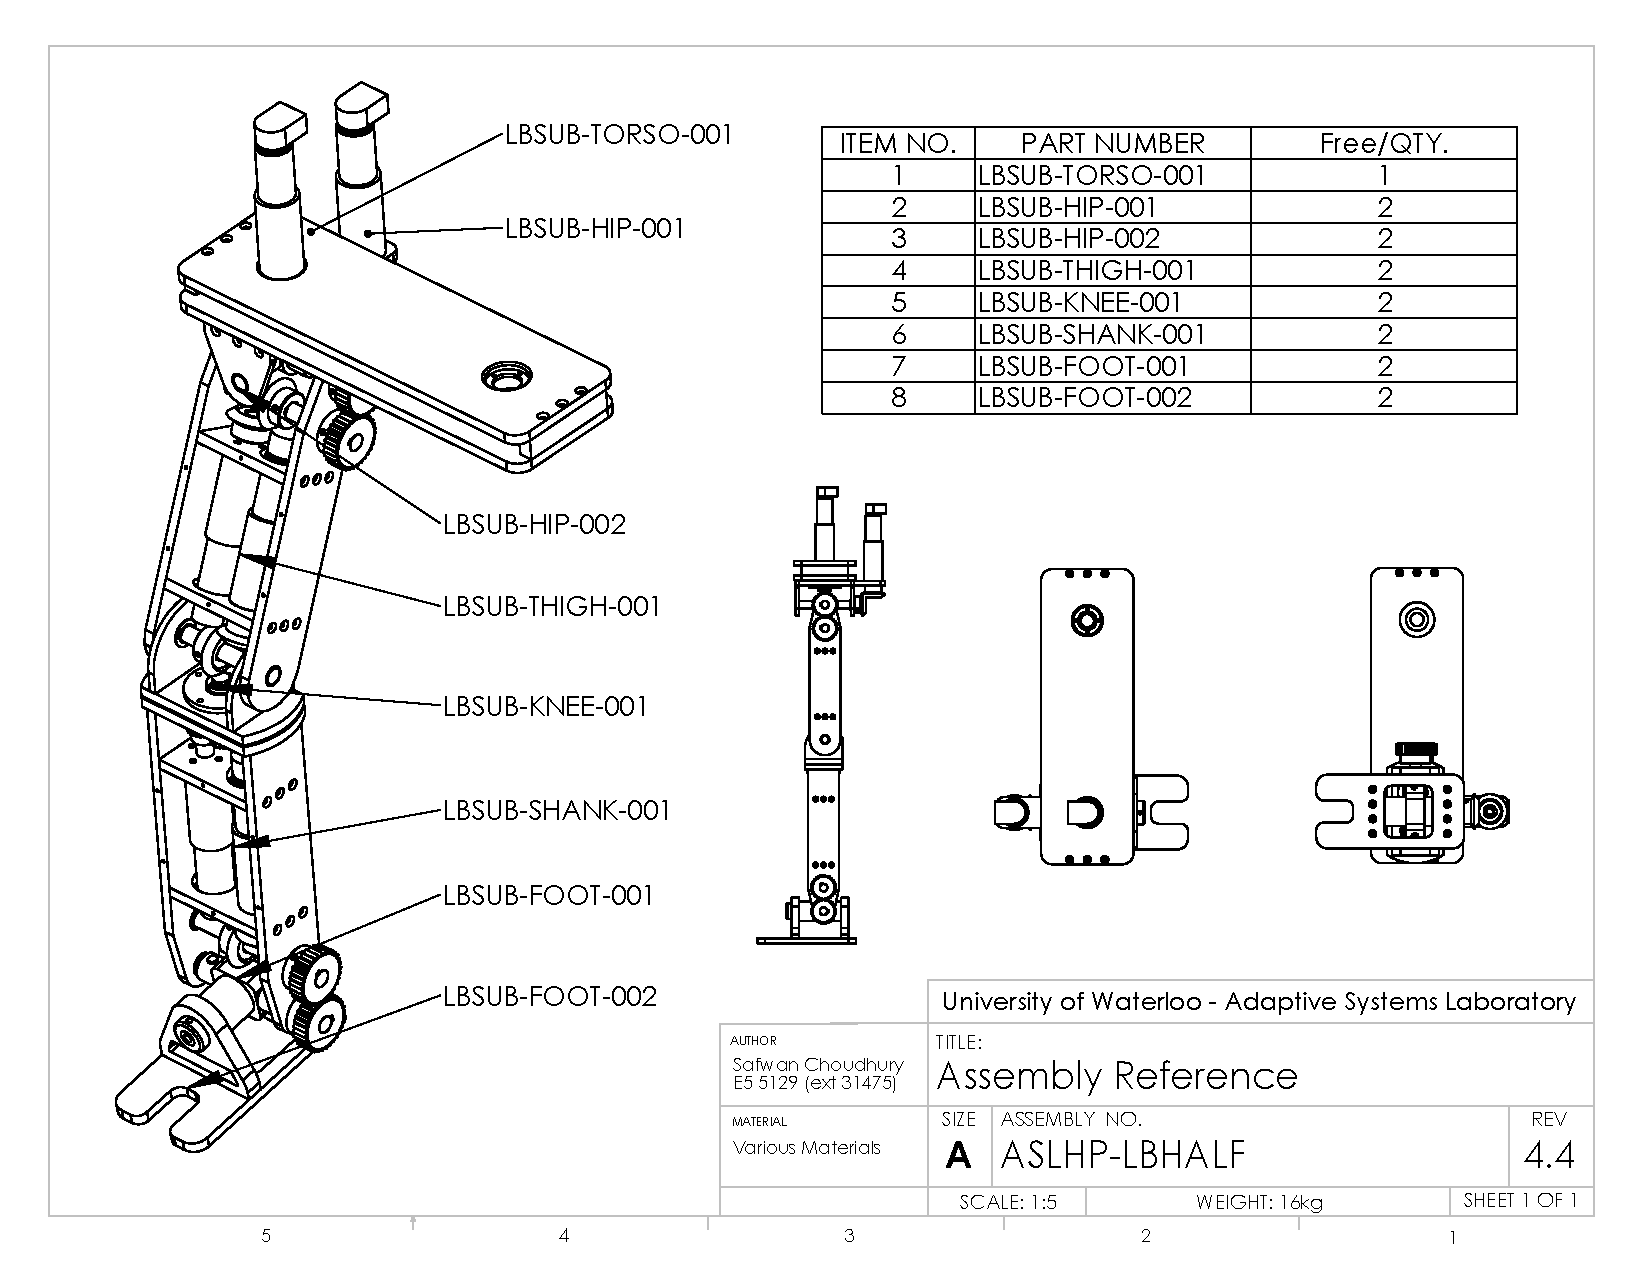
\includegraphics[scale=0.72,angle=90]{fig/drawings/aslhp-lbhalf.pdf}
	\end{center}
\end{figure}

\begin{figure}[!h]
	\begin{center}
    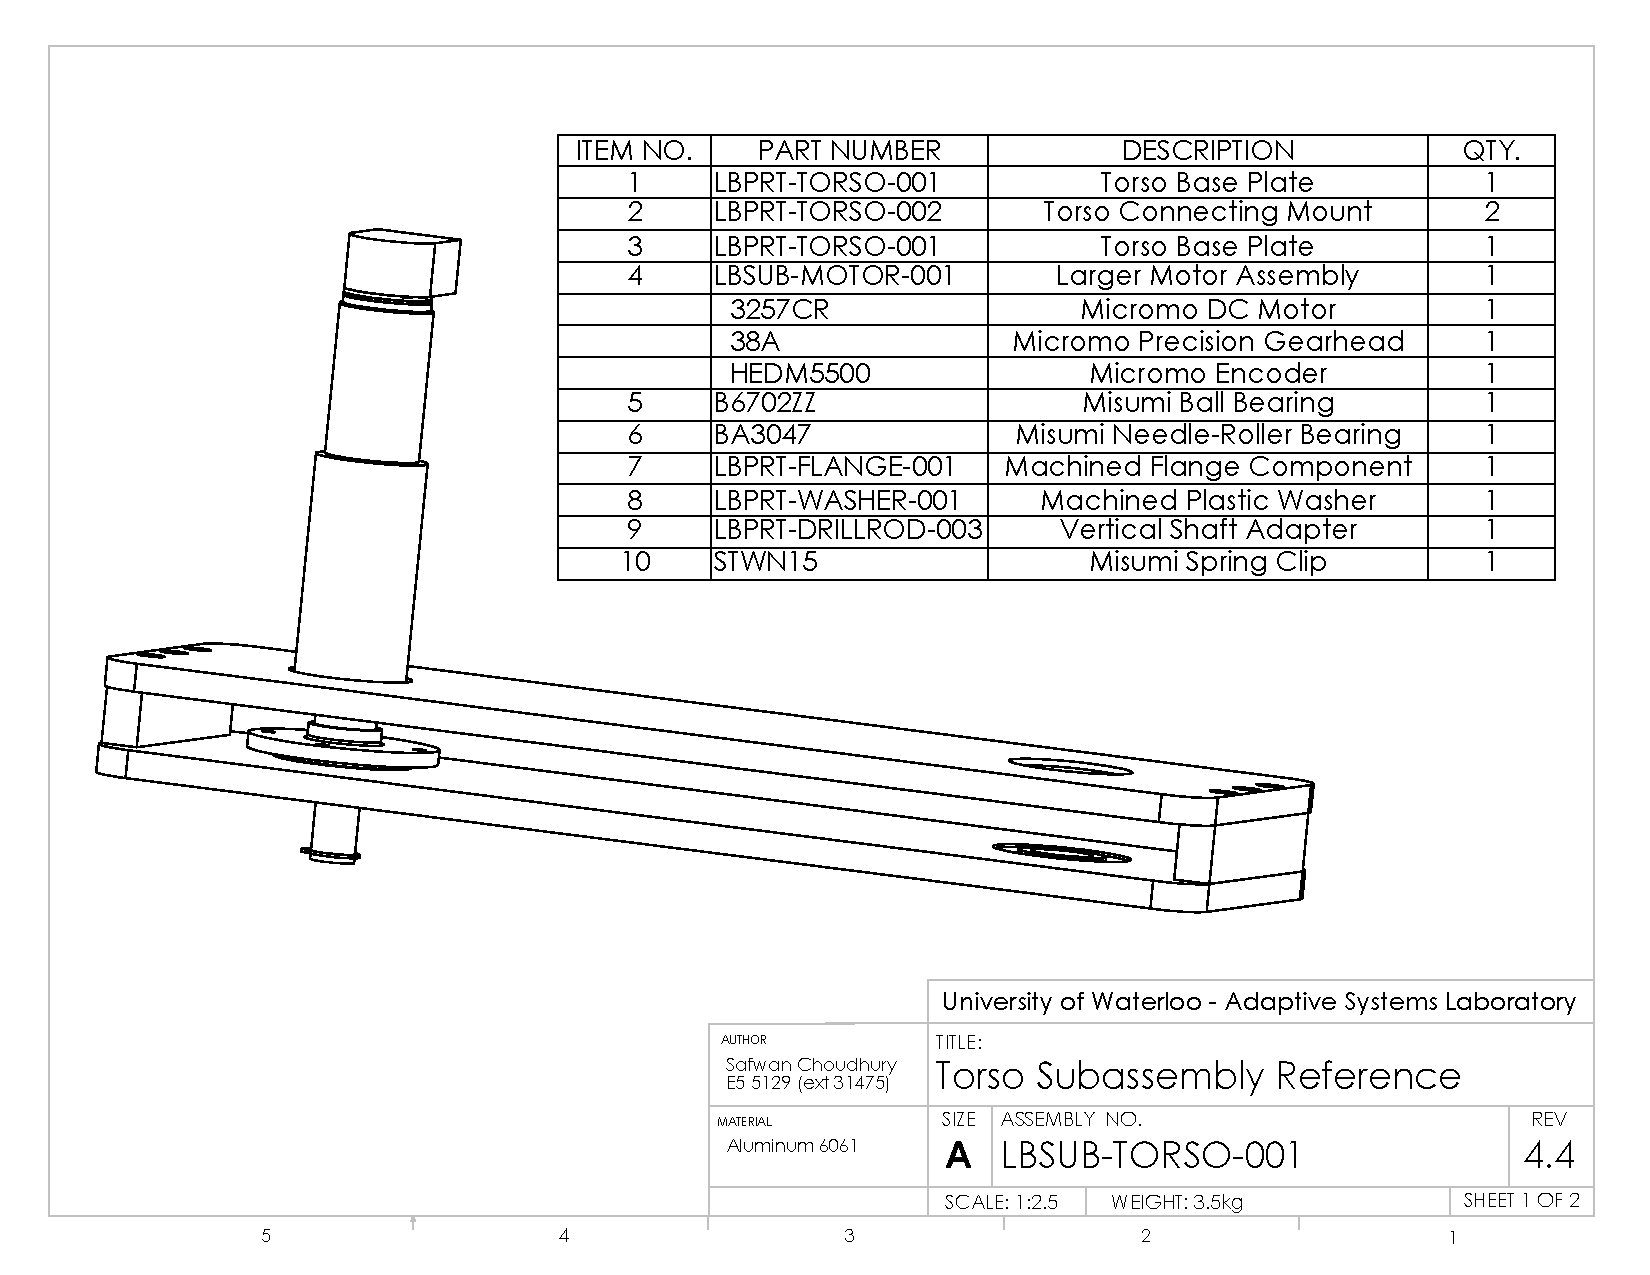
\includegraphics[scale=0.72,angle=90]{fig/drawings/lbsub-torso-001.pdf}
	\end{center}
\end{figure}

\begin{figure}[!h]
	\begin{center}
    \includegraphics[scale=0.72,angle=90,page=2]{fig/drawings/lbsub-torso-001.pdf}
	\end{center}
\end{figure}

\begin{figure}[!h]
	\begin{center}
    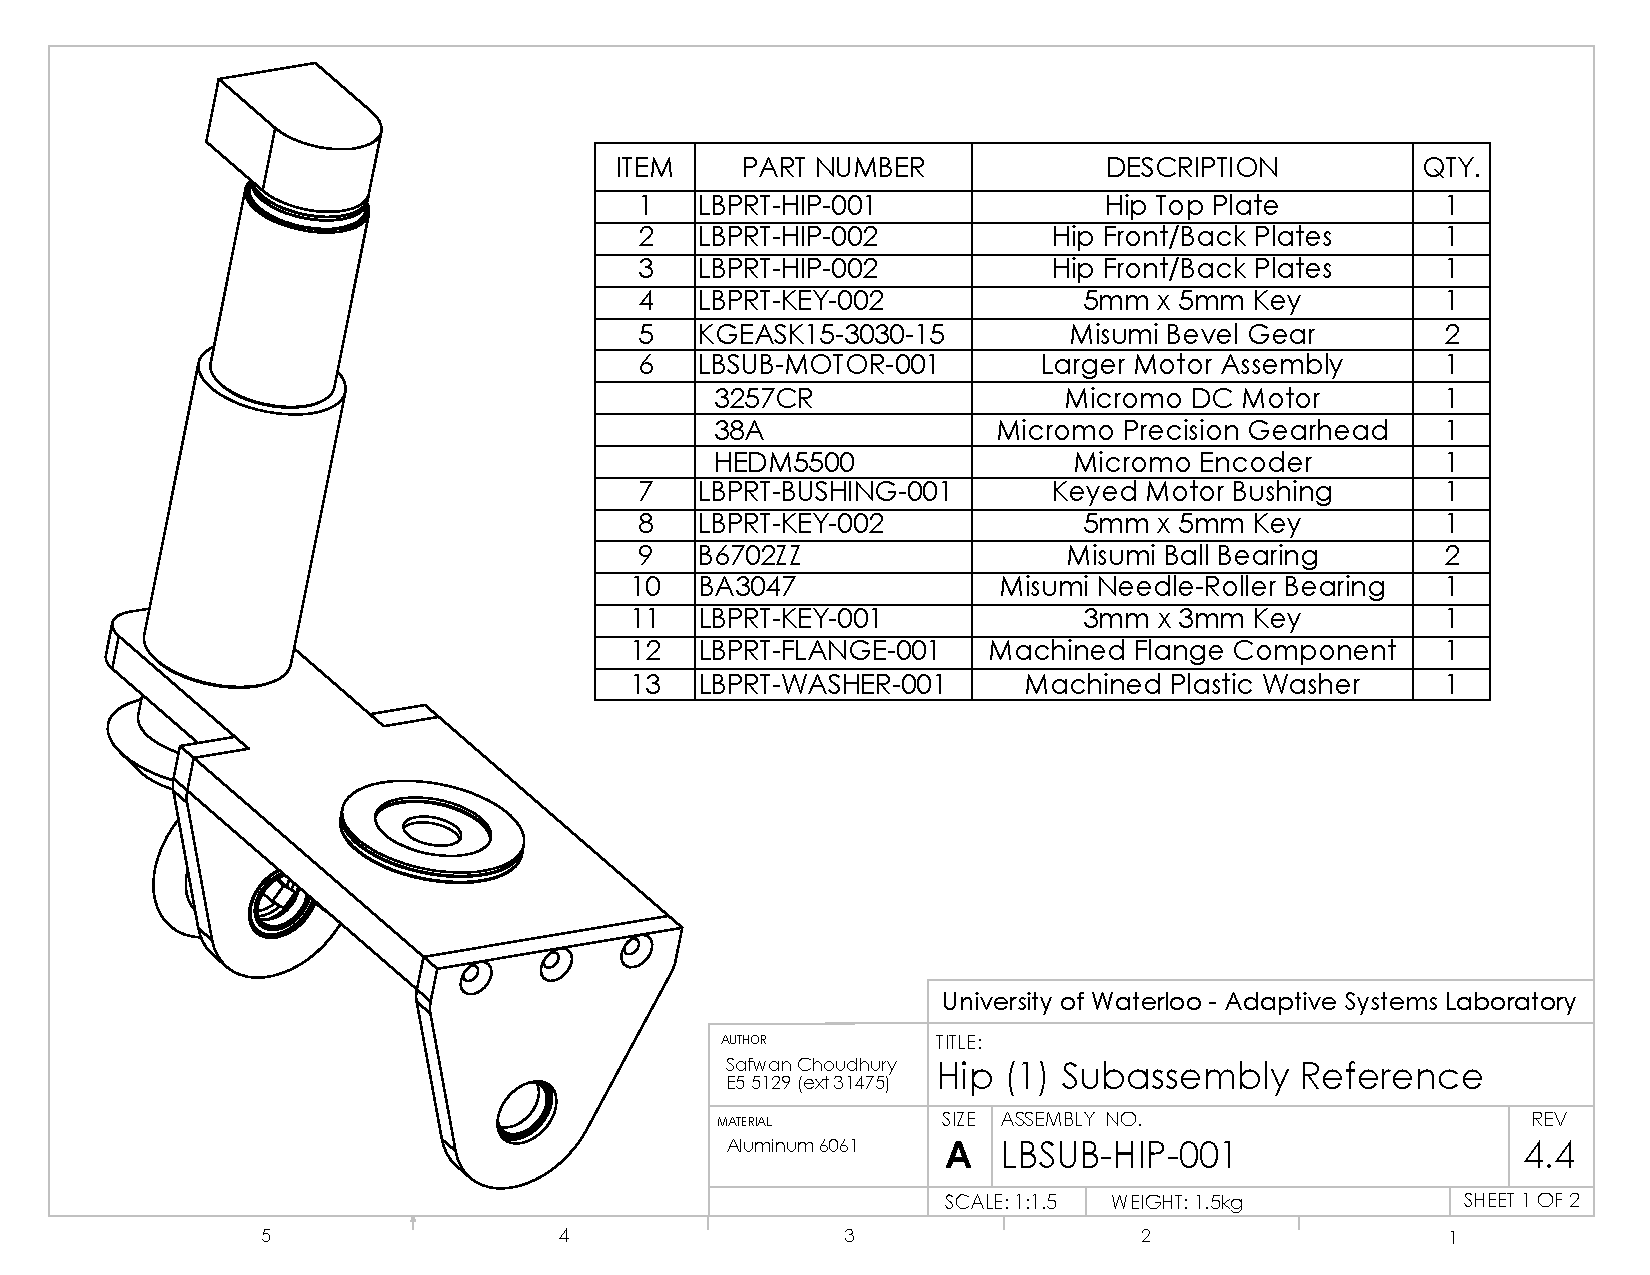
\includegraphics[scale=0.72,angle=90]{fig/drawings/lbsub-hip-001.pdf}
	\end{center}
\end{figure}

\begin{figure}[!h]
	\begin{center}
    \includegraphics[scale=0.72,angle=90,page=2]{fig/drawings/lbsub-hip-001.pdf}
	\end{center}
\end{figure}

\begin{figure}[!h]
	\begin{center}
    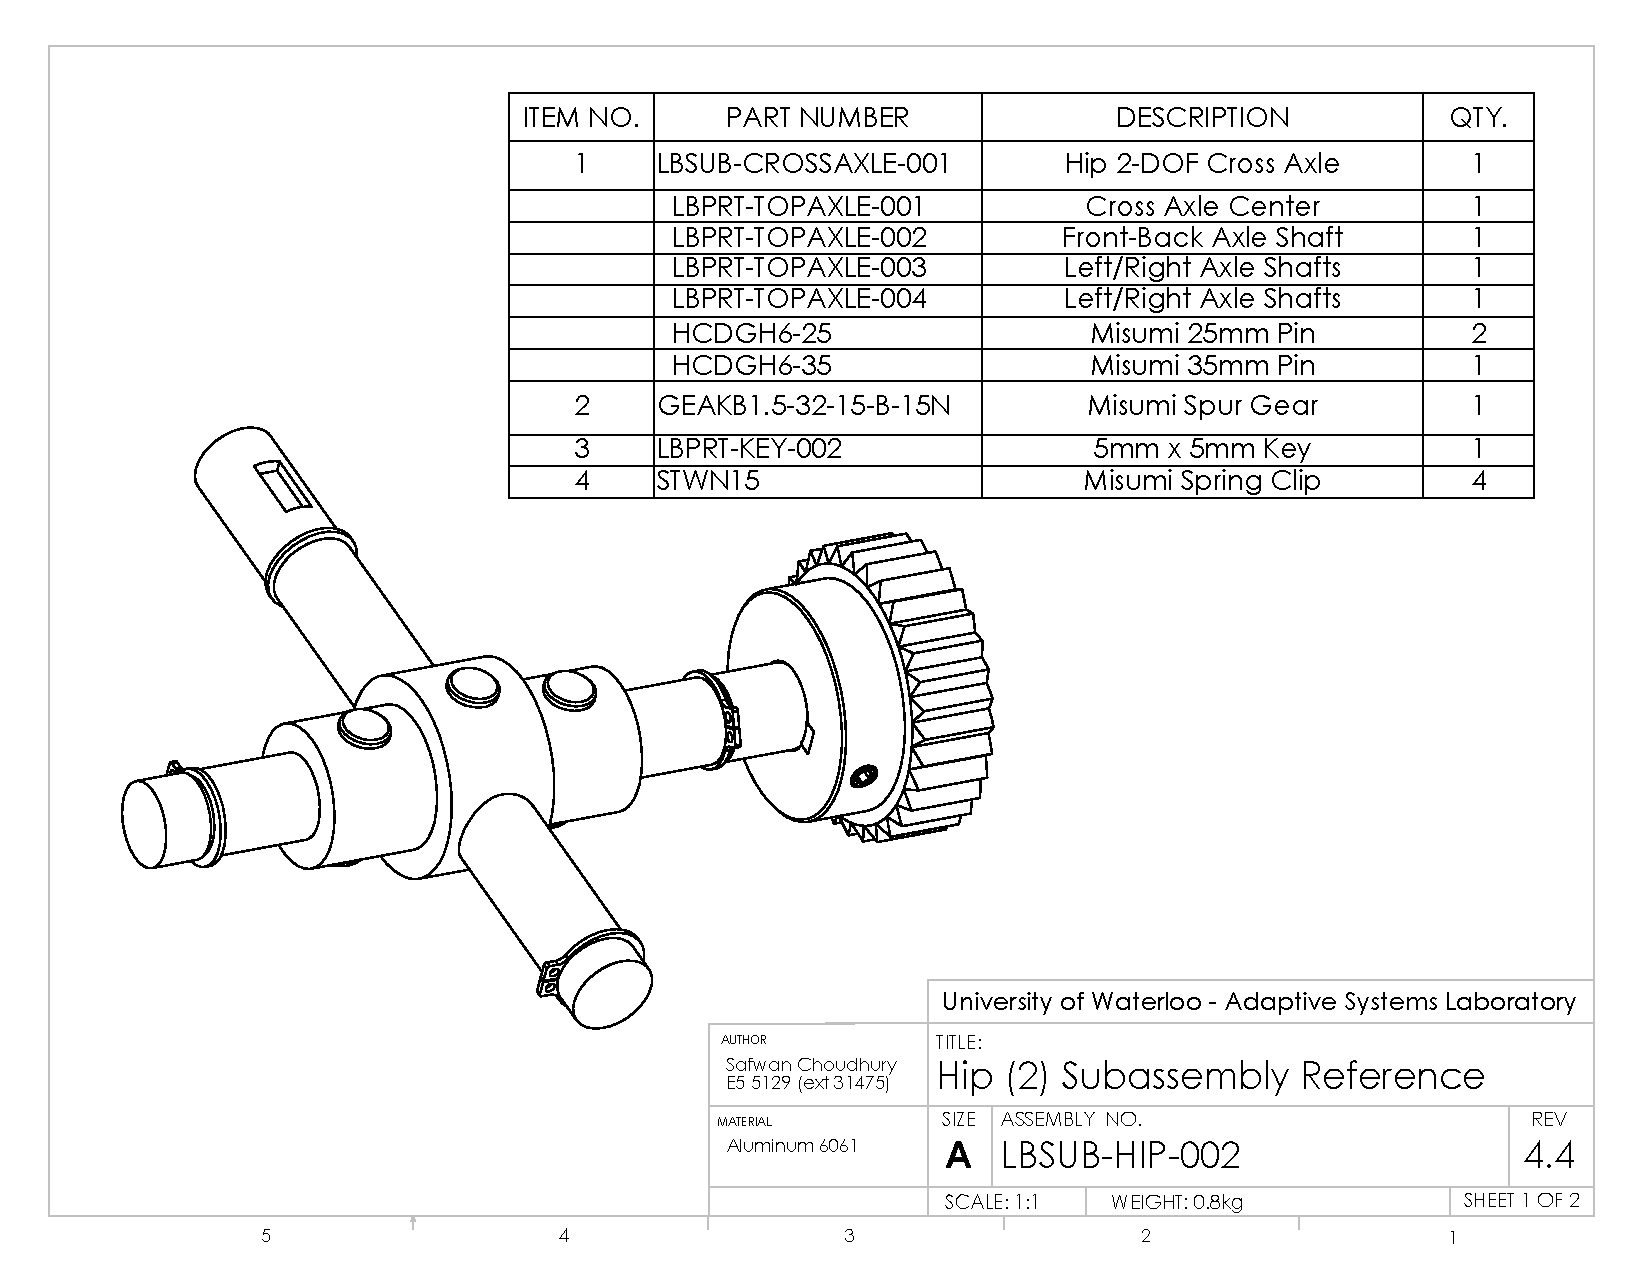
\includegraphics[scale=0.72,angle=90]{fig/drawings/lbsub-hip-002.pdf}
	\end{center}
\end{figure}

\begin{figure}[!h]
	\begin{center}
    \includegraphics[scale=0.72,angle=90,page=2]{fig/drawings/lbsub-hip-002.pdf}
	\end{center}
\end{figure}


\begin{figure}[!h]
	\begin{center}
    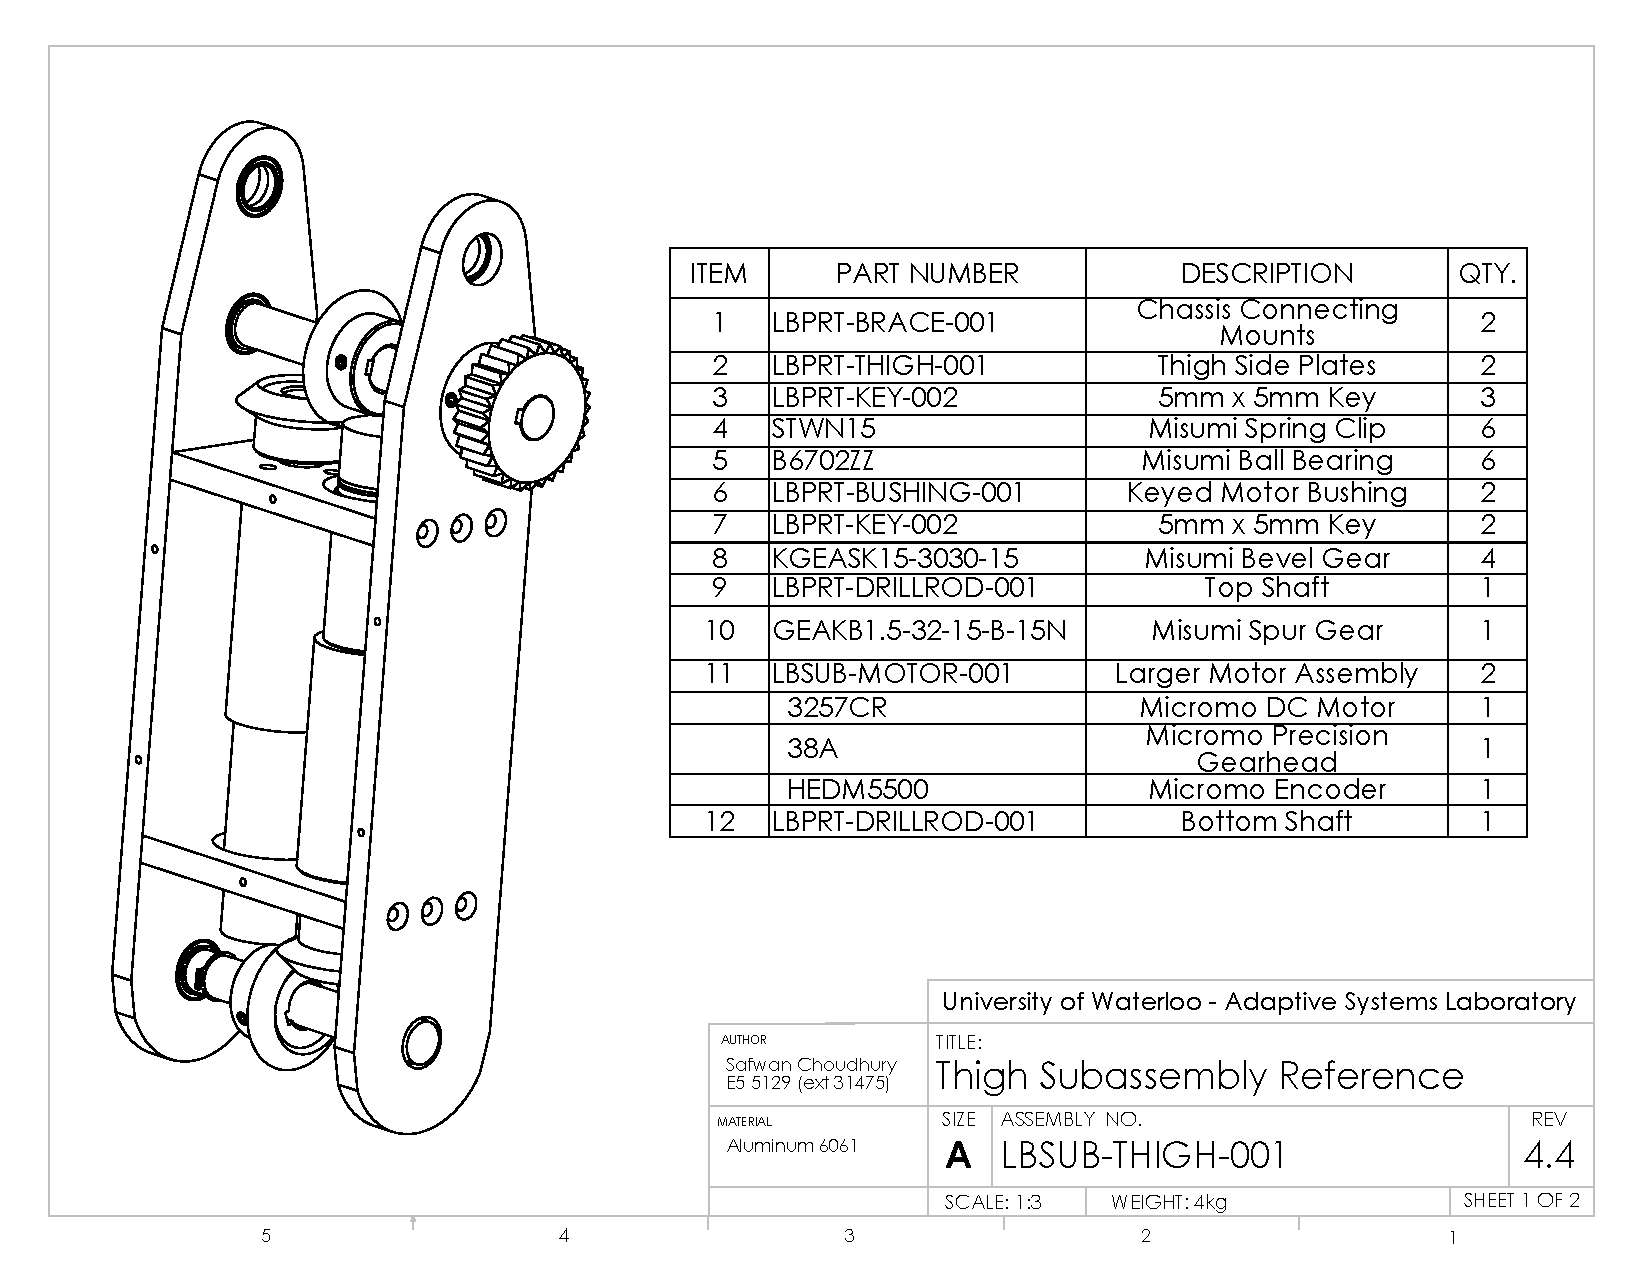
\includegraphics[scale=0.72,angle=90]{fig/drawings/lbsub-thigh-001.pdf}
	\end{center}
\end{figure}

\begin{figure}[!h]
	\begin{center}
    \includegraphics[scale=0.72,angle=90,page=2]{fig/drawings/lbsub-thigh-001.pdf}
	\end{center}
\end{figure}

\begin{figure}[!h]
	\begin{center}
    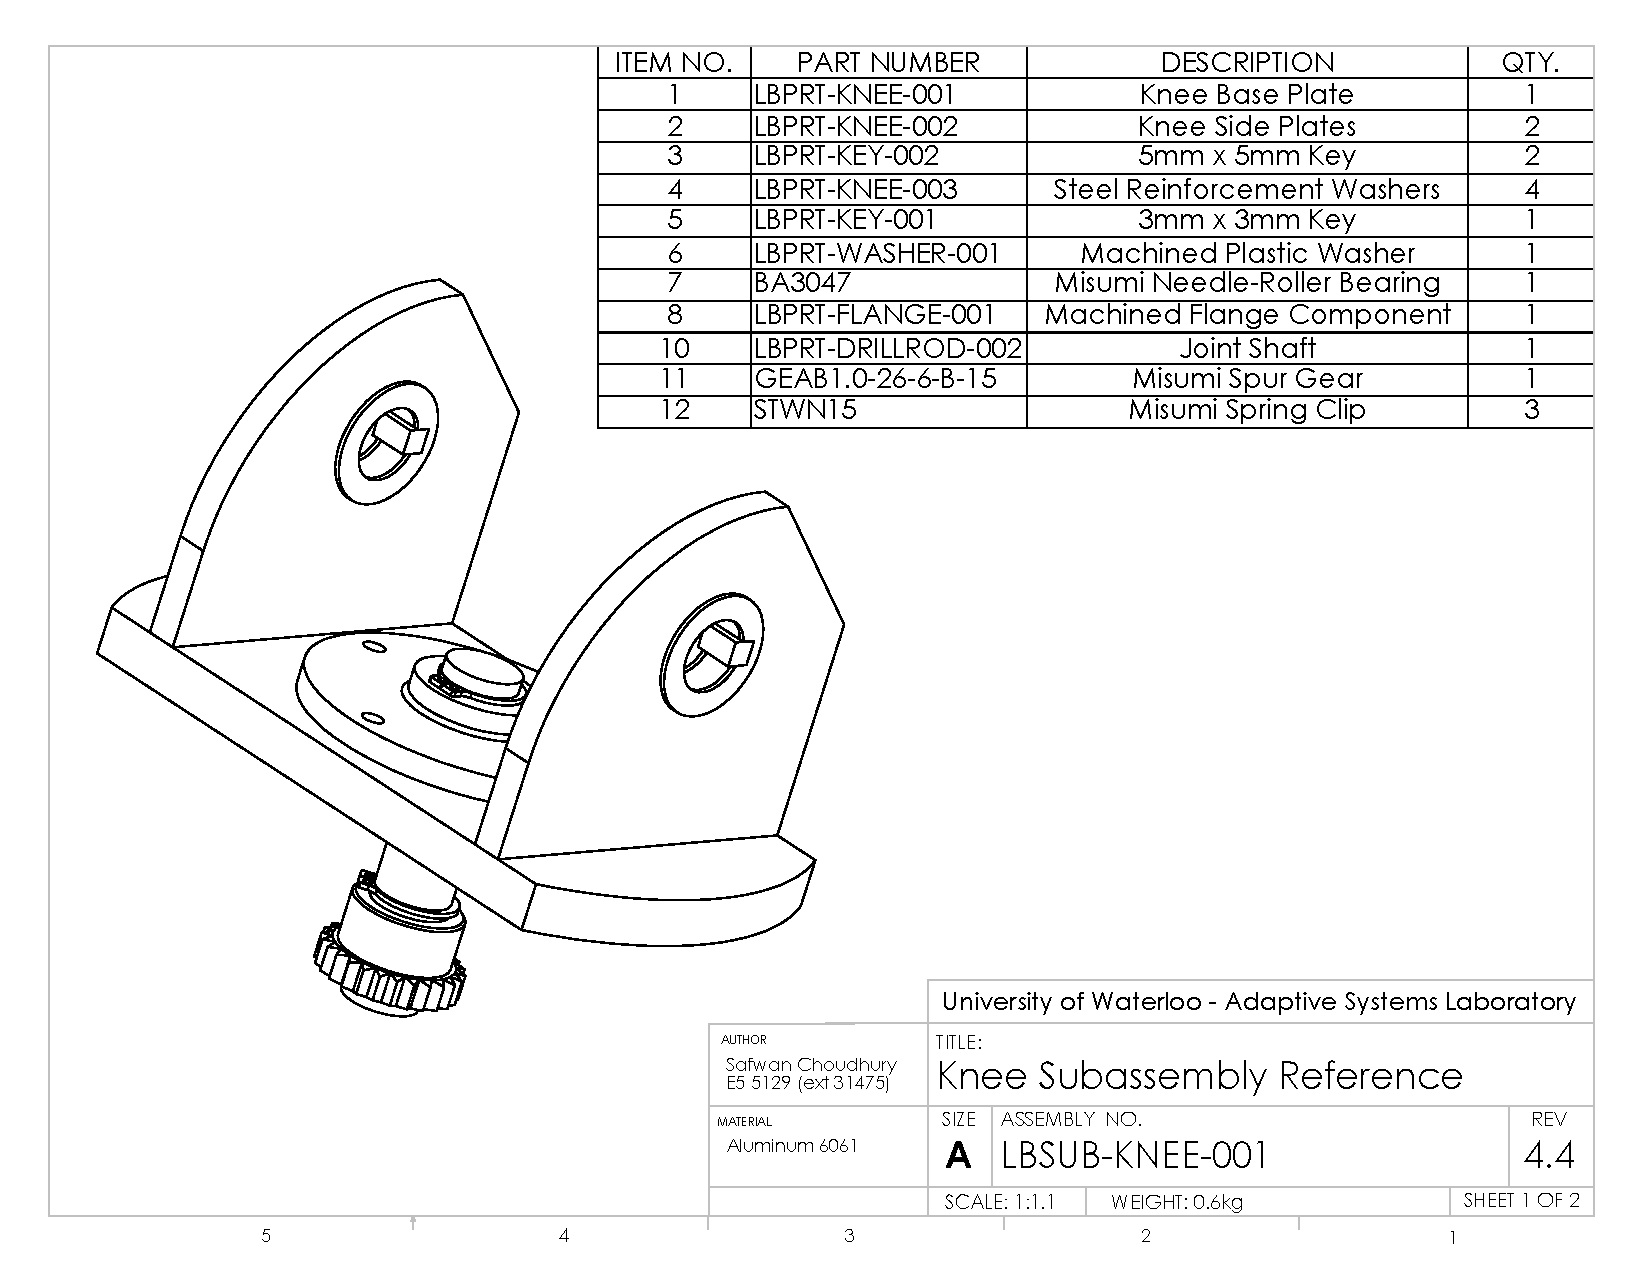
\includegraphics[scale=0.72,angle=90]{fig/drawings/lbsub-knee-001.pdf}
	\end{center}
\end{figure}

\begin{figure}[!h]
	\begin{center}
    \includegraphics[scale=0.72,angle=90,page=2]{fig/drawings/lbsub-knee-001.pdf}
	\end{center}
\end{figure}

\begin{figure}[!h]
	\begin{center}
    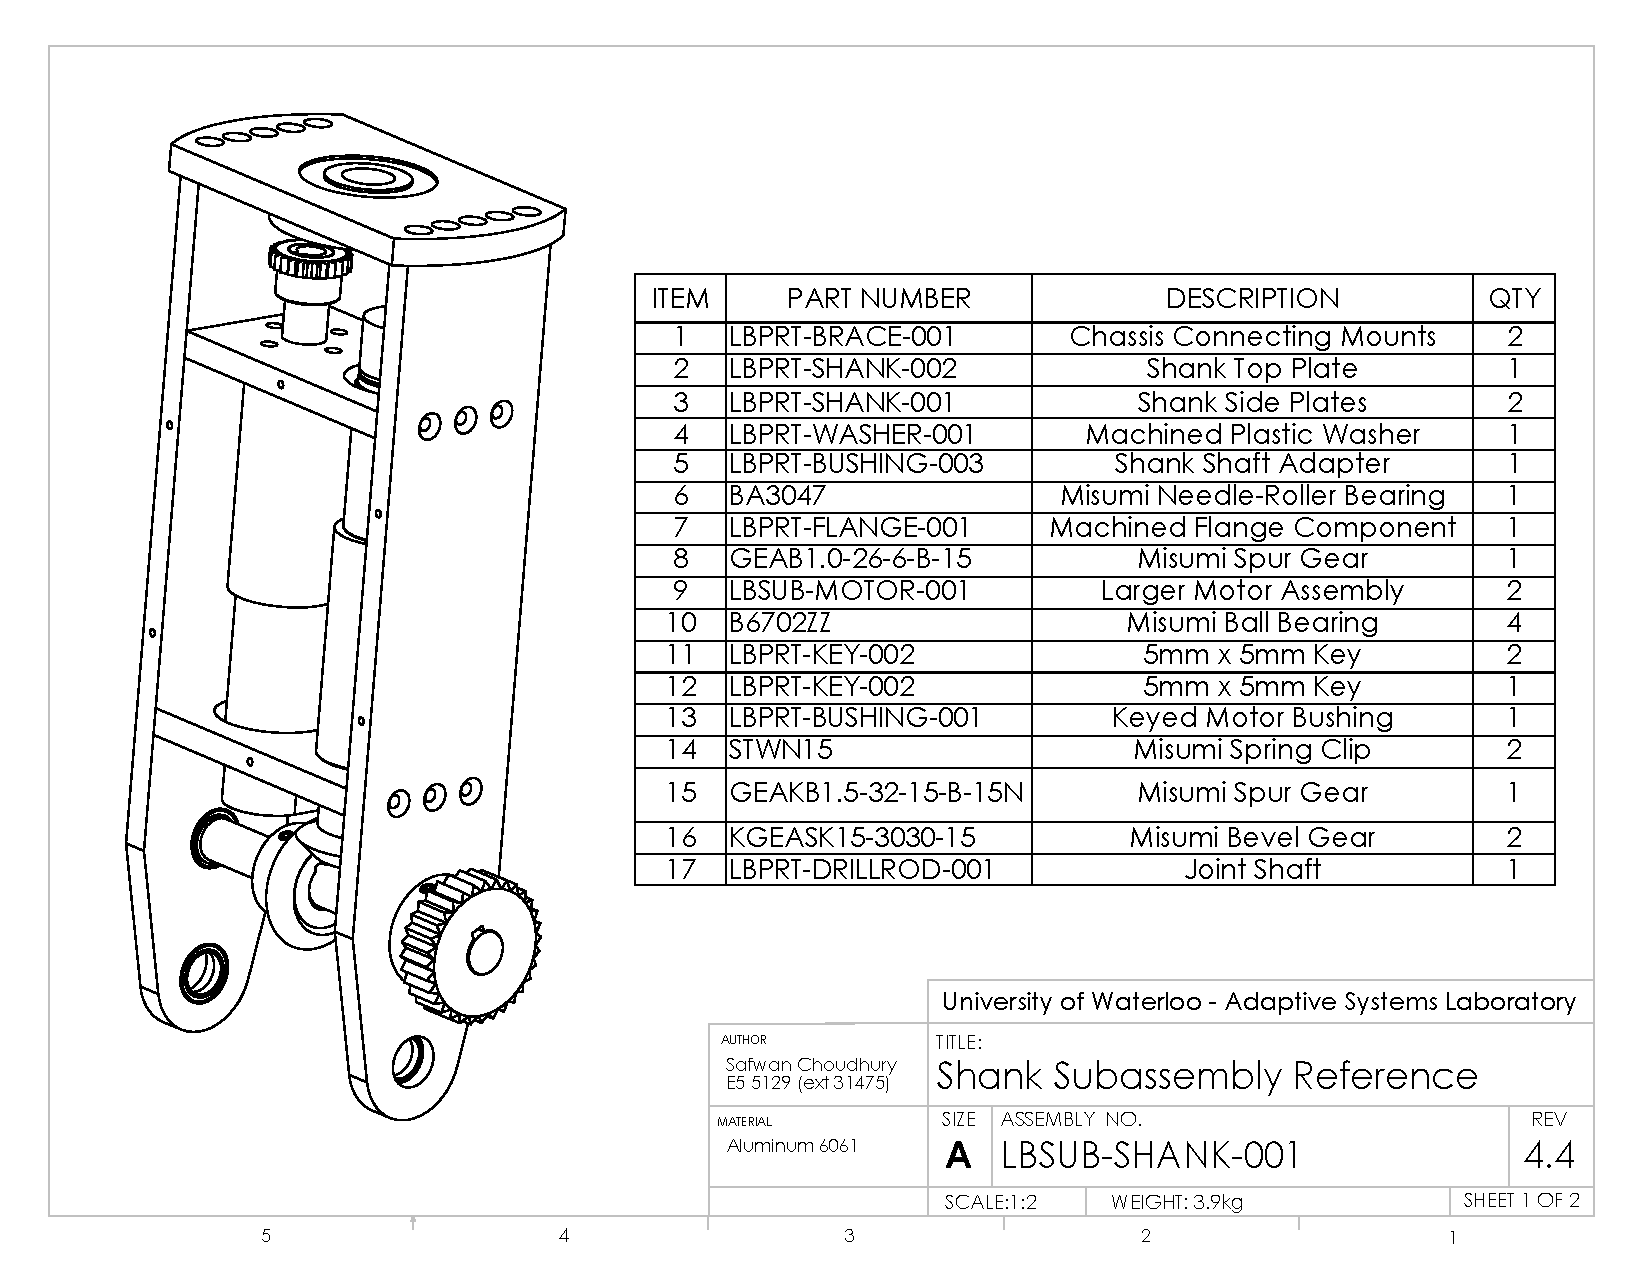
\includegraphics[scale=0.72,angle=90]{fig/drawings/lbsub-shank-001.pdf}
	\end{center}
\end{figure}

\begin{figure}[!h]
	\begin{center}
    \includegraphics[scale=0.72,angle=90,page=2]{fig/drawings/lbsub-shank-001.pdf}
	\end{center}
\end{figure}

\begin{figure}[!h]
	\begin{center}
    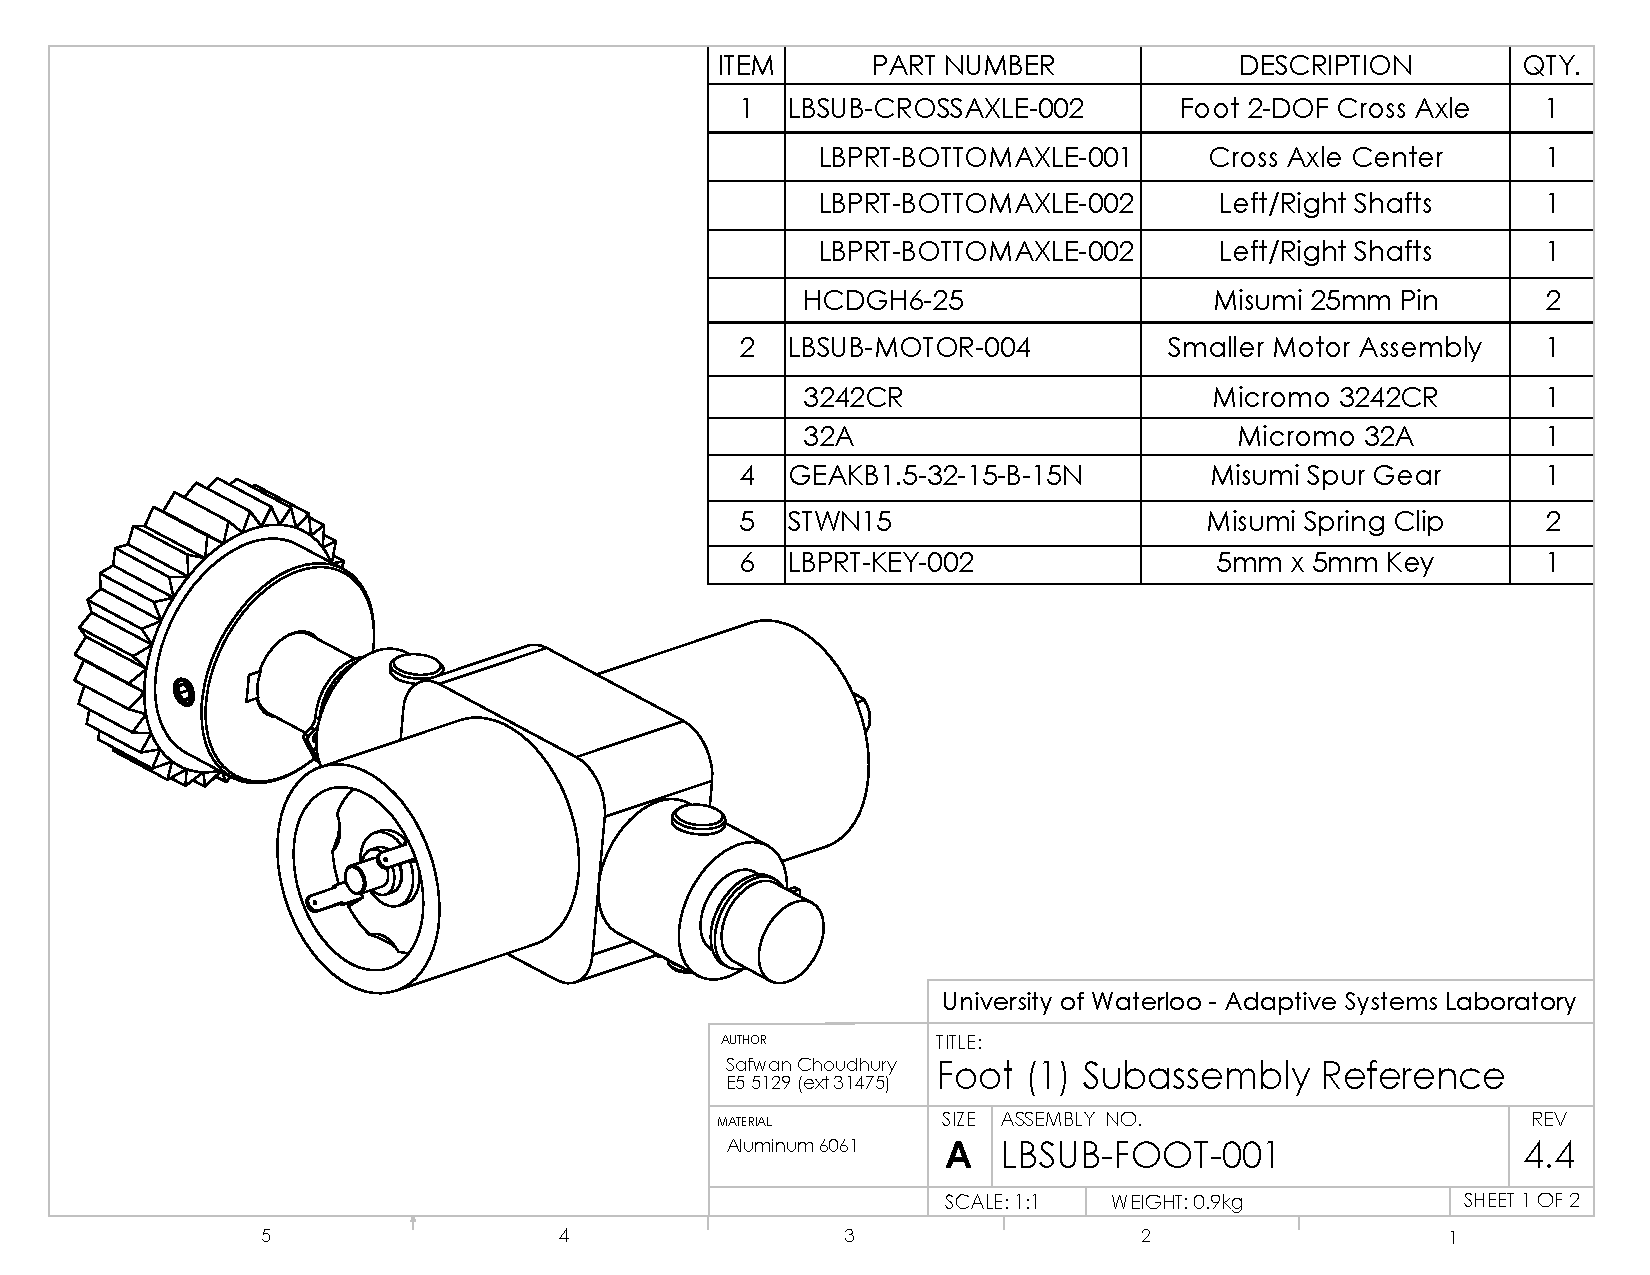
\includegraphics[scale=0.72,angle=90]{fig/drawings/lbsub-foot-001.pdf}
	\end{center}
\end{figure}

\begin{figure}[!h]
	\begin{center}
    \includegraphics[scale=0.72,angle=90,page=2]{fig/drawings/lbsub-foot-001.pdf}
	\end{center}
\end{figure}

\begin{figure}[!h]
	\begin{center}
    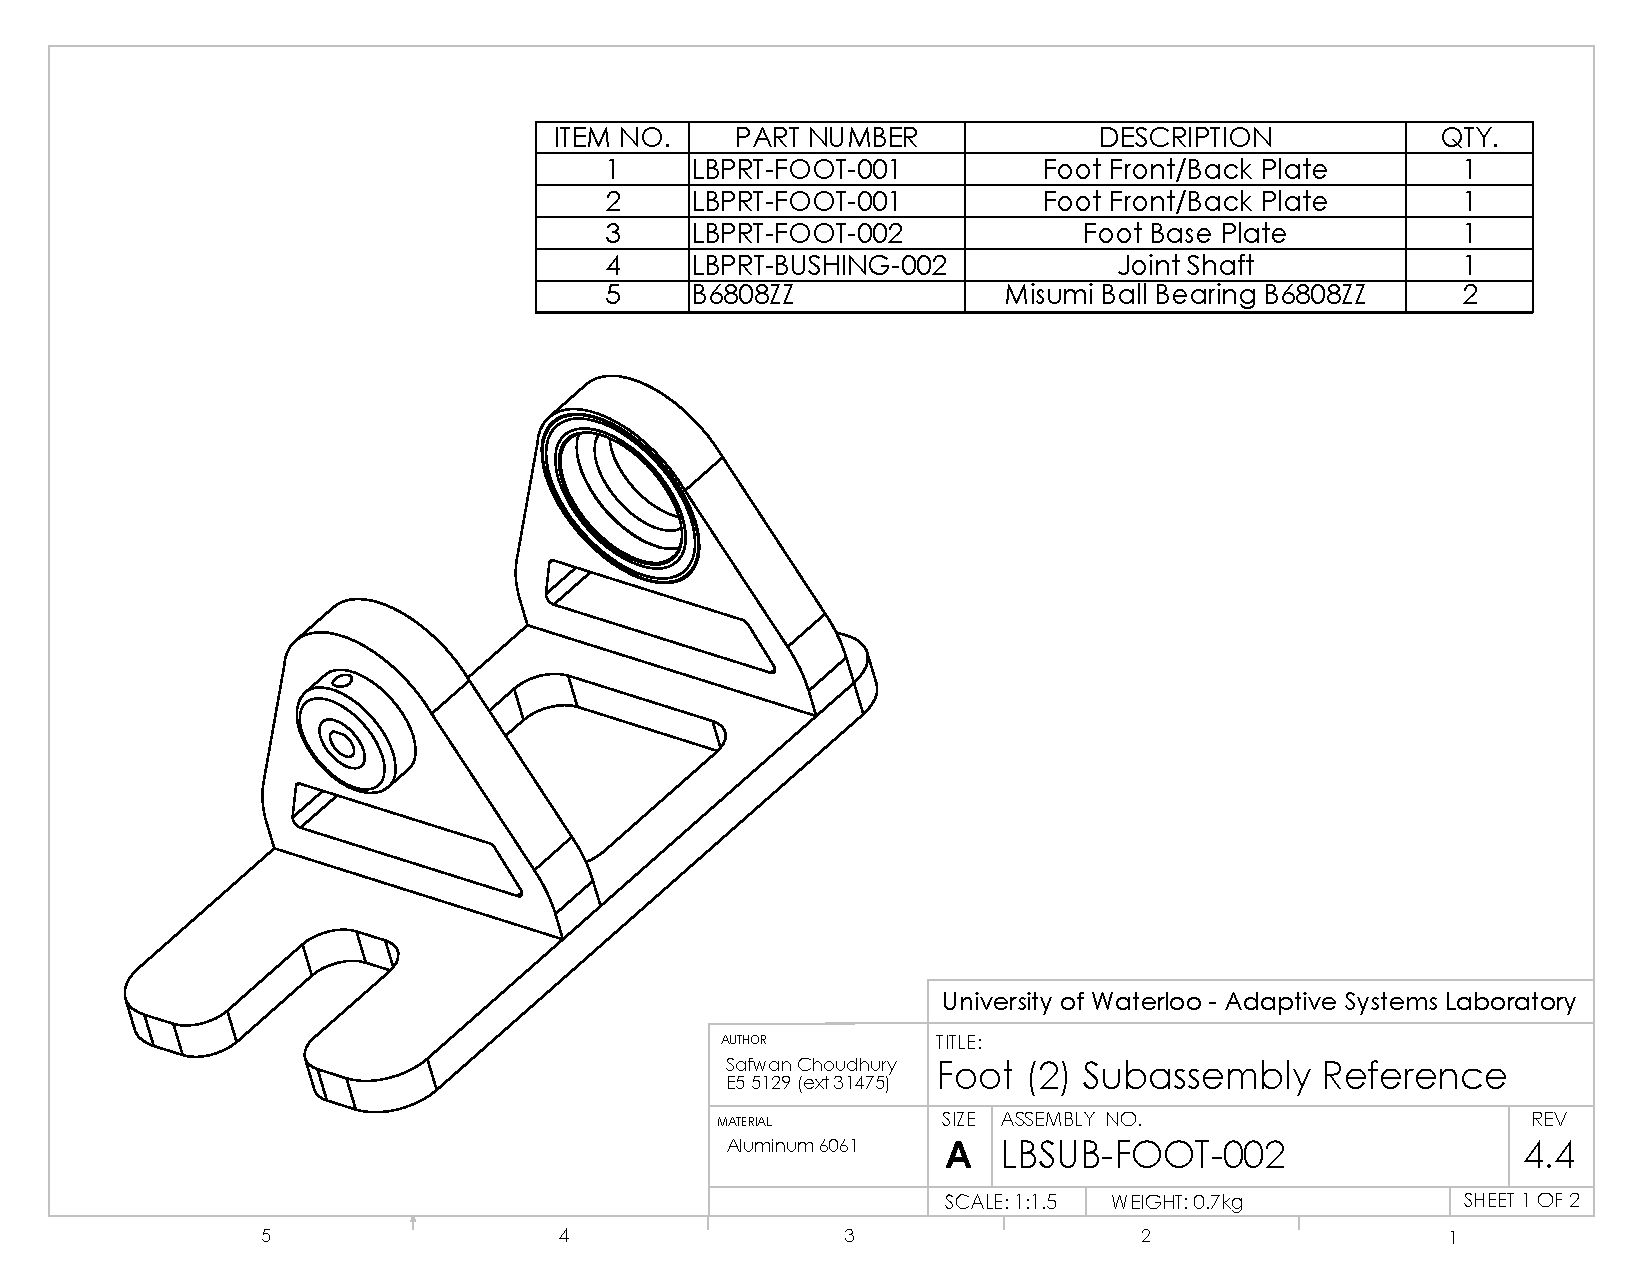
\includegraphics[scale=0.72,angle=90]{fig/drawings/lbsub-foot-002.pdf}
	\end{center}
\end{figure}

\begin{figure}[!h]
	\begin{center}
    \includegraphics[scale=0.72,angle=90,page=2]{fig/drawings/lbsub-foot-002.pdf}
	\end{center}
\end{figure}

\clearpage

\section{Walking Frame} 
\label{app:framecad}
The supporting frame was designed for fixed base and (tethered) walking experiments. 

% Supporting components were supplied by McMaster Carr\footnote{http://www.mcmaster.com}. 

\textbf{Fixed Configuration}

\begin{figure}[!h]
	\begin{center}
    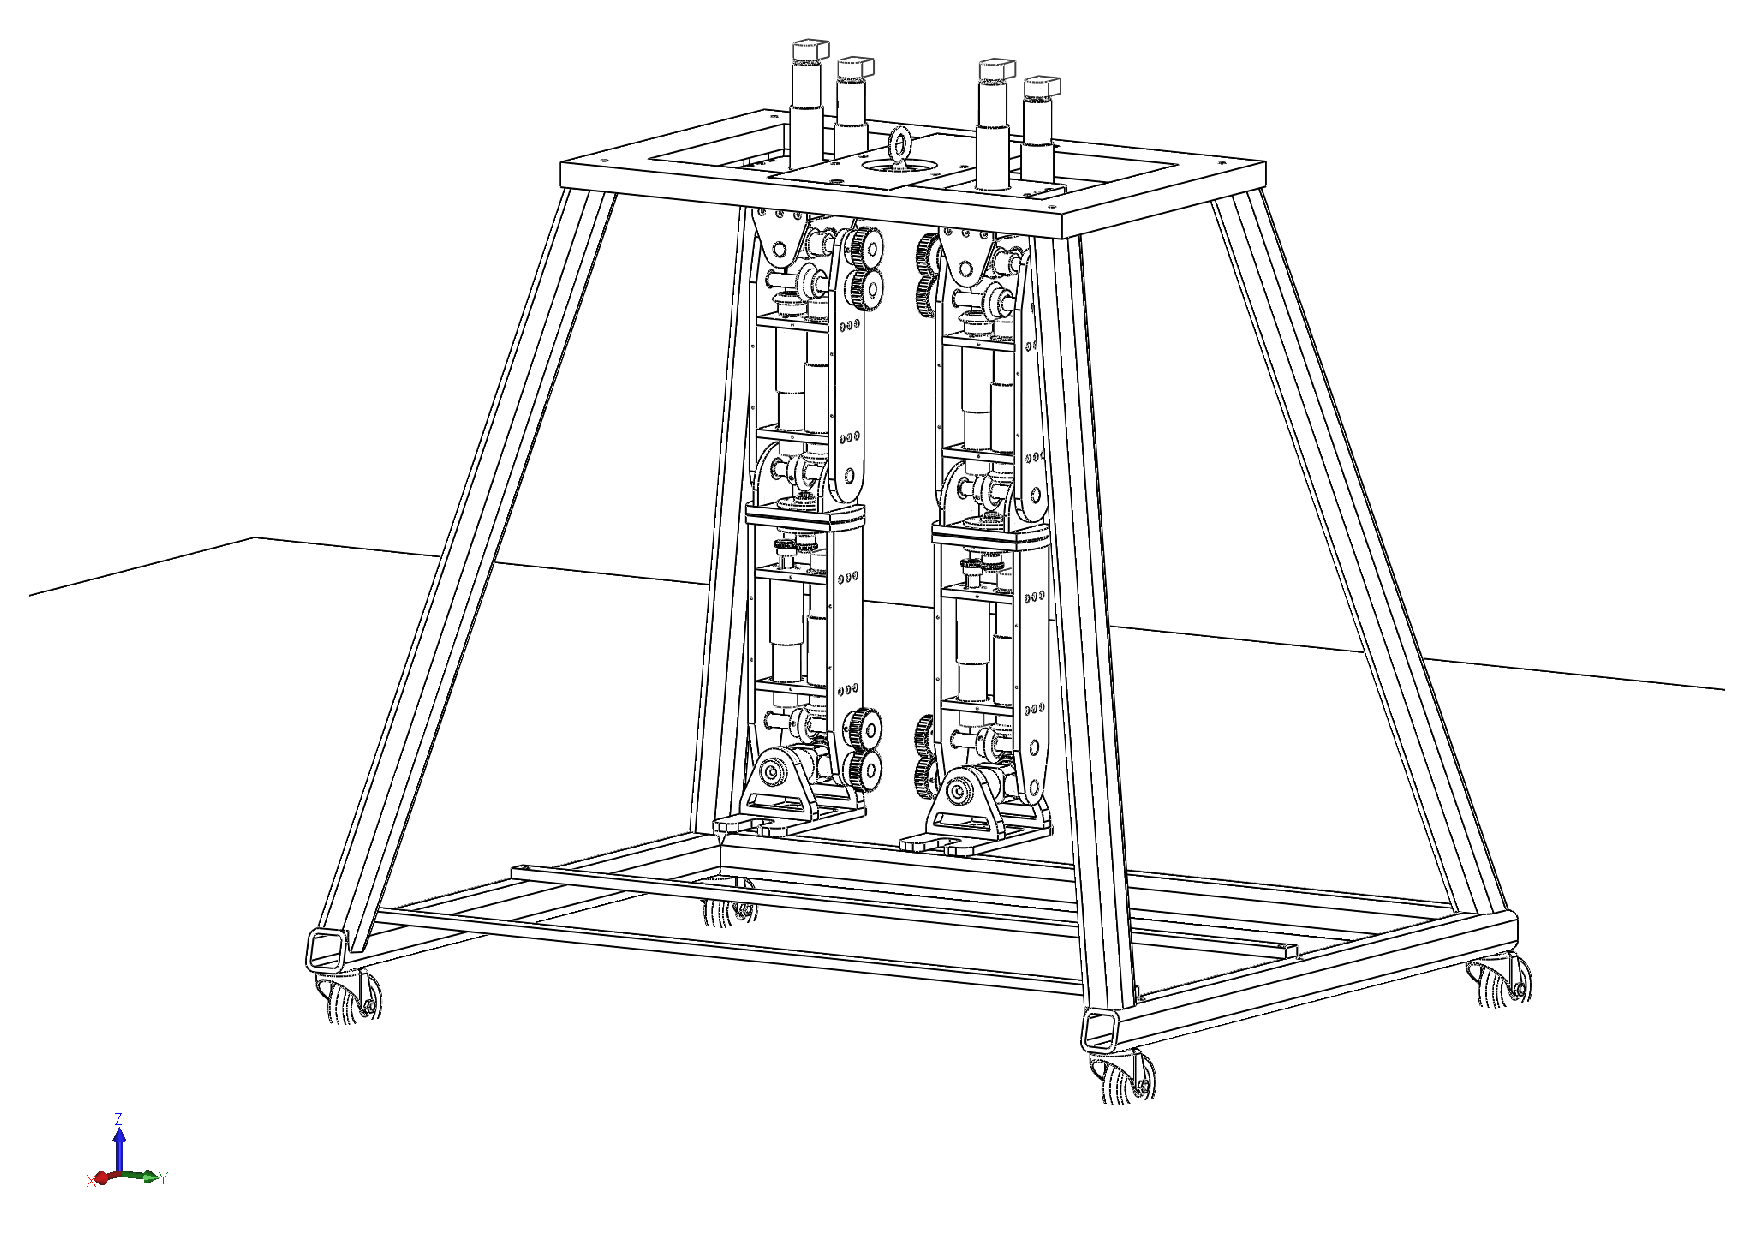
\includegraphics[trim = 5mm 20mm 5mm 5mm,clip,width=10cm]{fig/drawings/frame-fixed.pdf}
	\end{center}
\end{figure}

\textbf{Walking Configuration}

\begin{figure}[!h]
	\begin{center}
    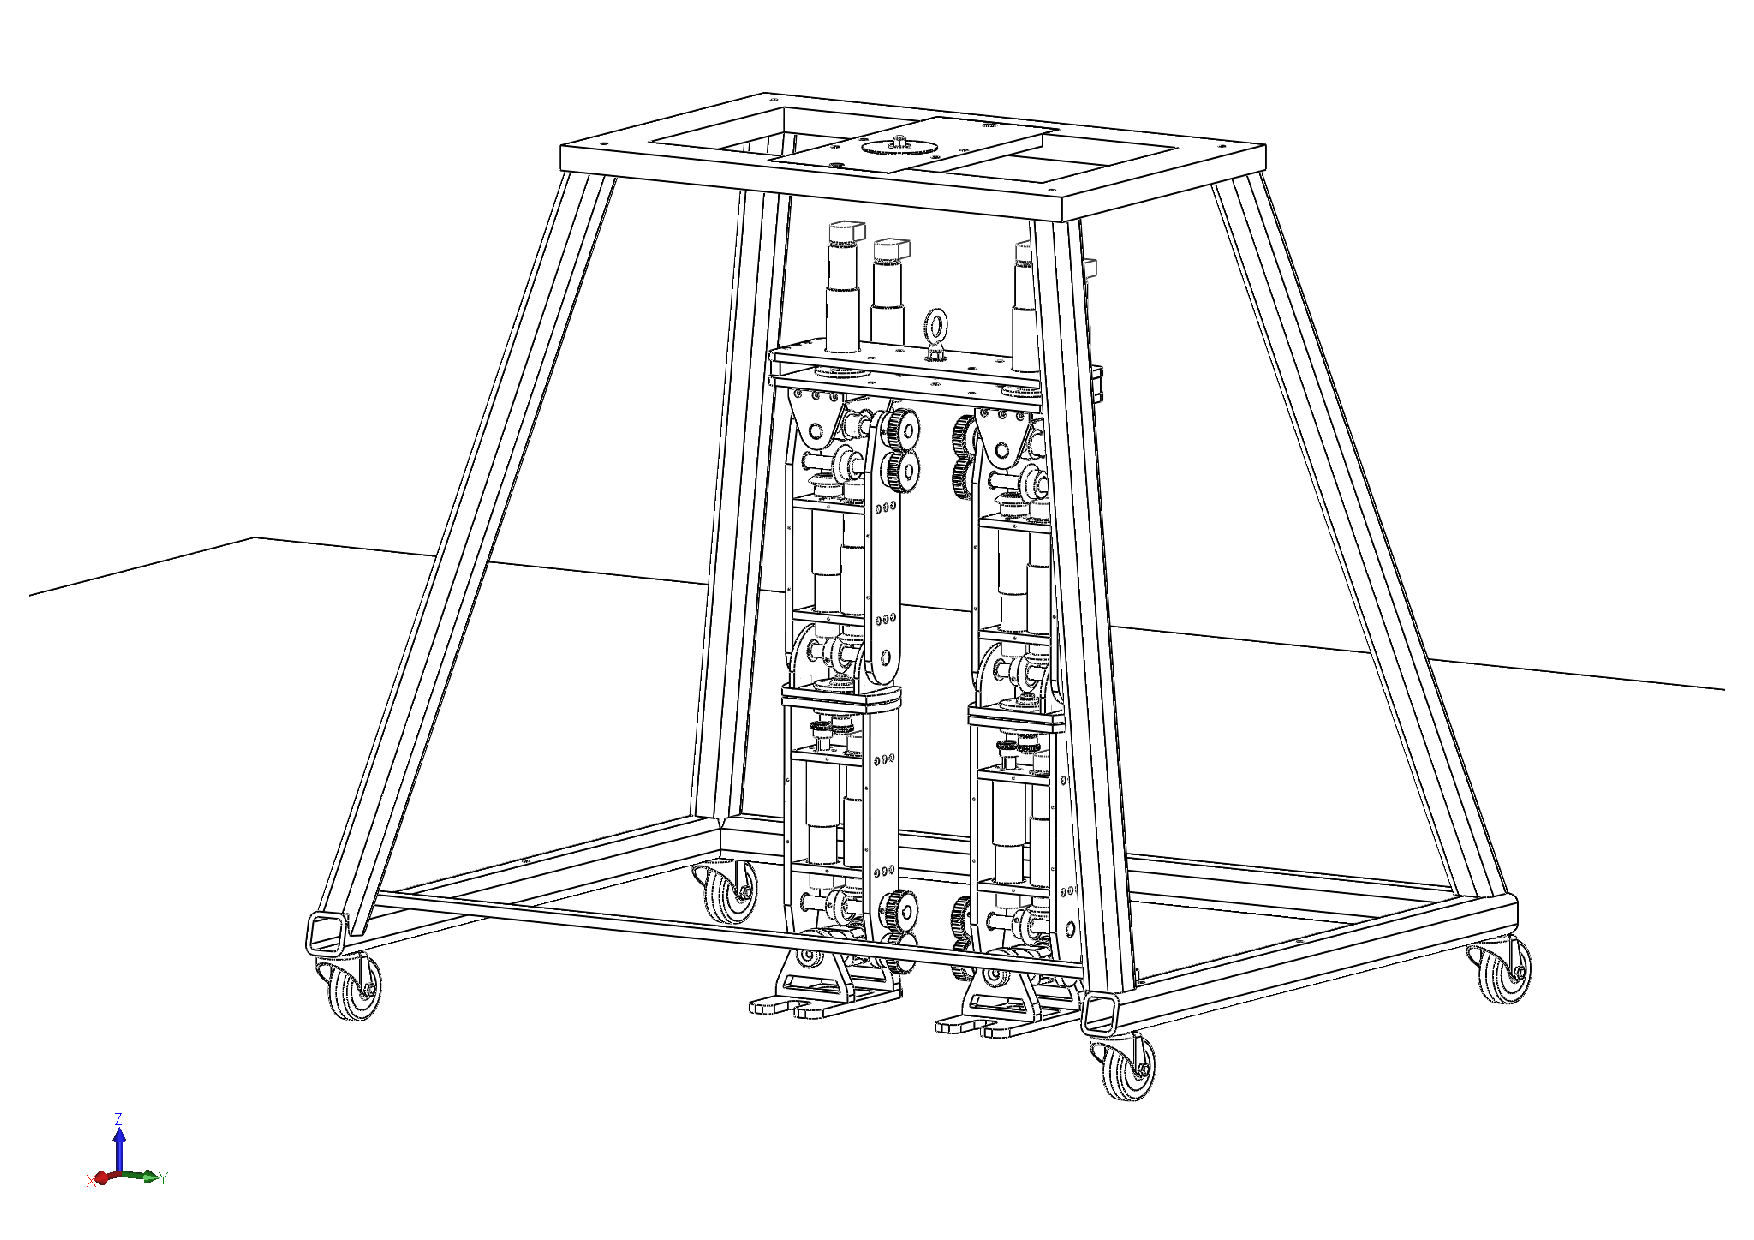
\includegraphics[trim = 5mm 20mm 5mm 5mm,clip,width=10cm]{fig/drawings/frame-walking.pdf}
	\end{center}
\end{figure}

\begin{figure}[!h]
	\begin{center}
    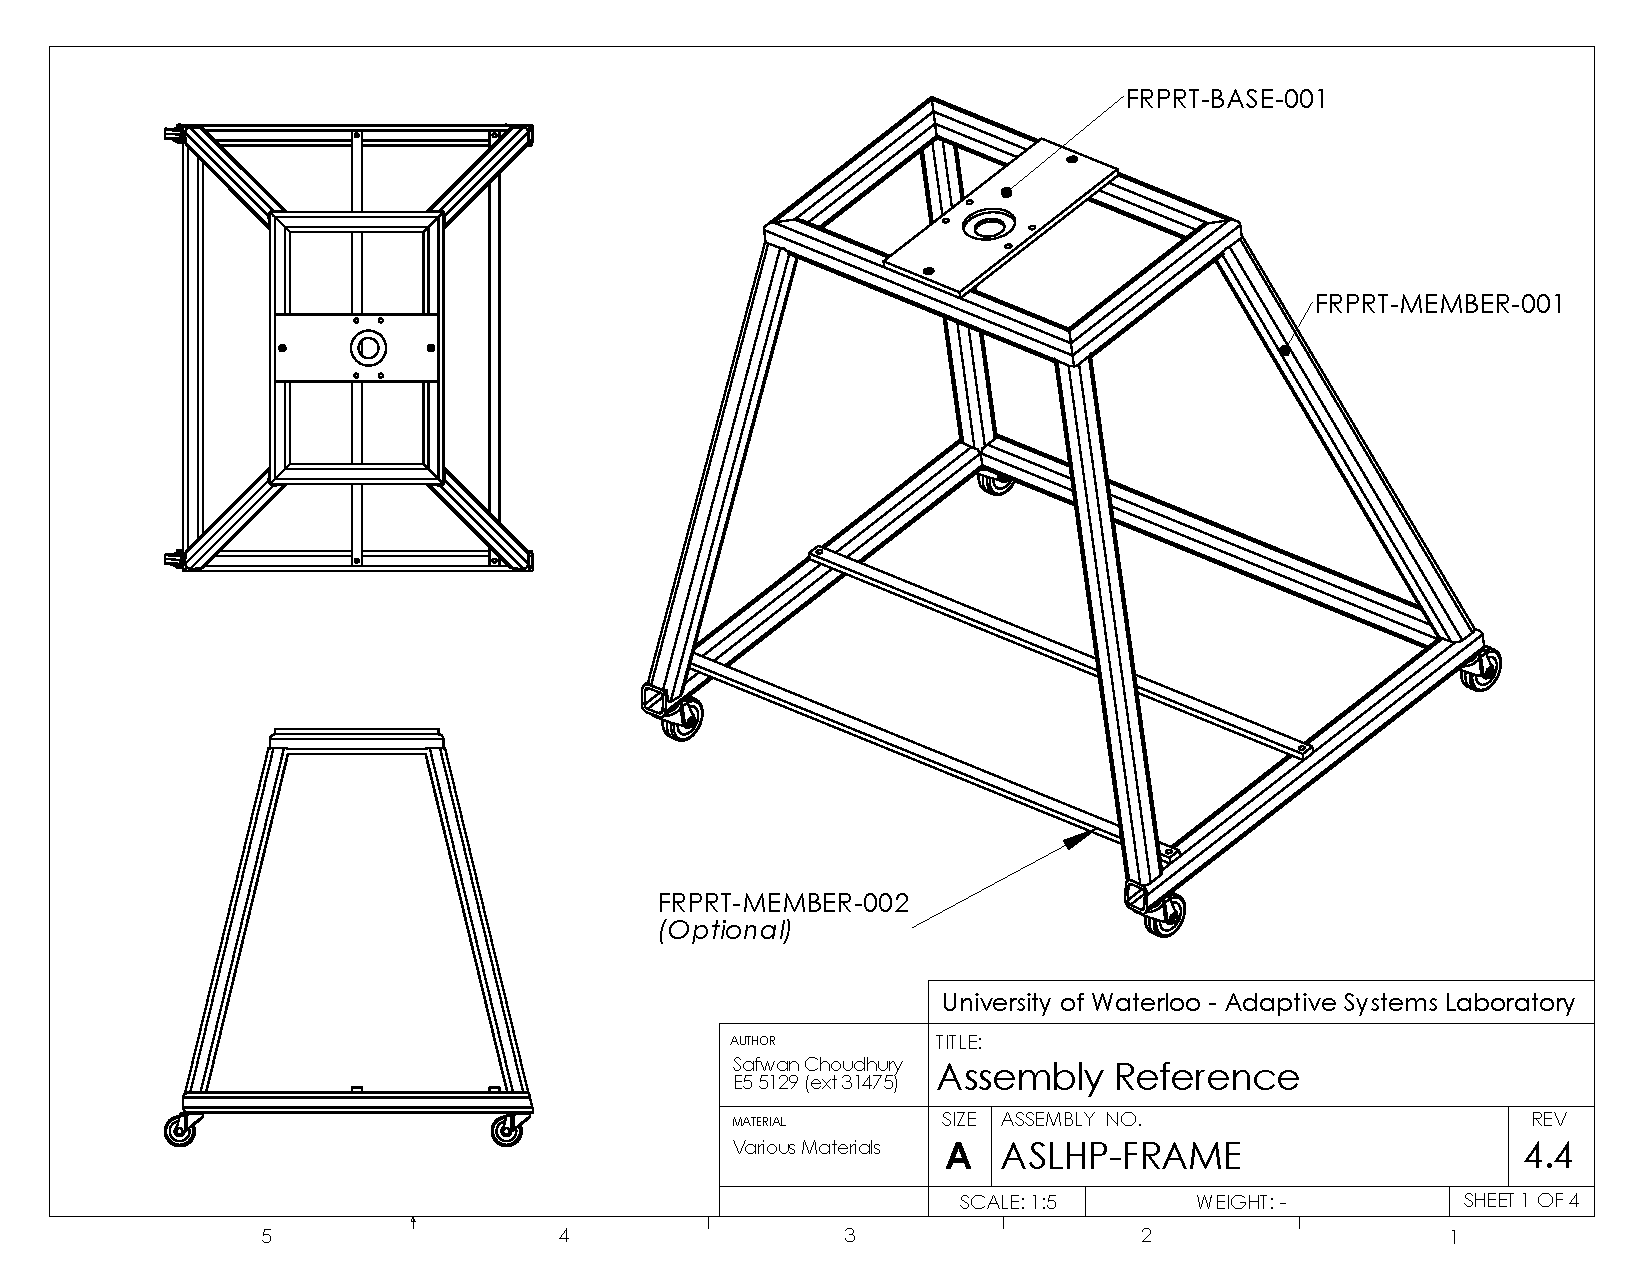
\includegraphics[scale=0.72,angle=90]{fig/drawings/aslhp-frame.pdf}
	\end{center}
\end{figure}

\begin{figure}[!h]
	\begin{center}
    \includegraphics[scale=0.72,angle=90,page=2]{fig/drawings/aslhp-frame.pdf}
	\end{center}
\end{figure}